\chapter{Architektur}

    \section{Aufteilung in die Pakete}

    \noindent Das System besteht aus einem \gls{Client}- und \gls{Server}-Teil, die miteinander mittels HTTP Requests kommunizieren. (Abbildung \ref{fig:arch_package_division})
    
    \begin{figure}[h]
        \centering
        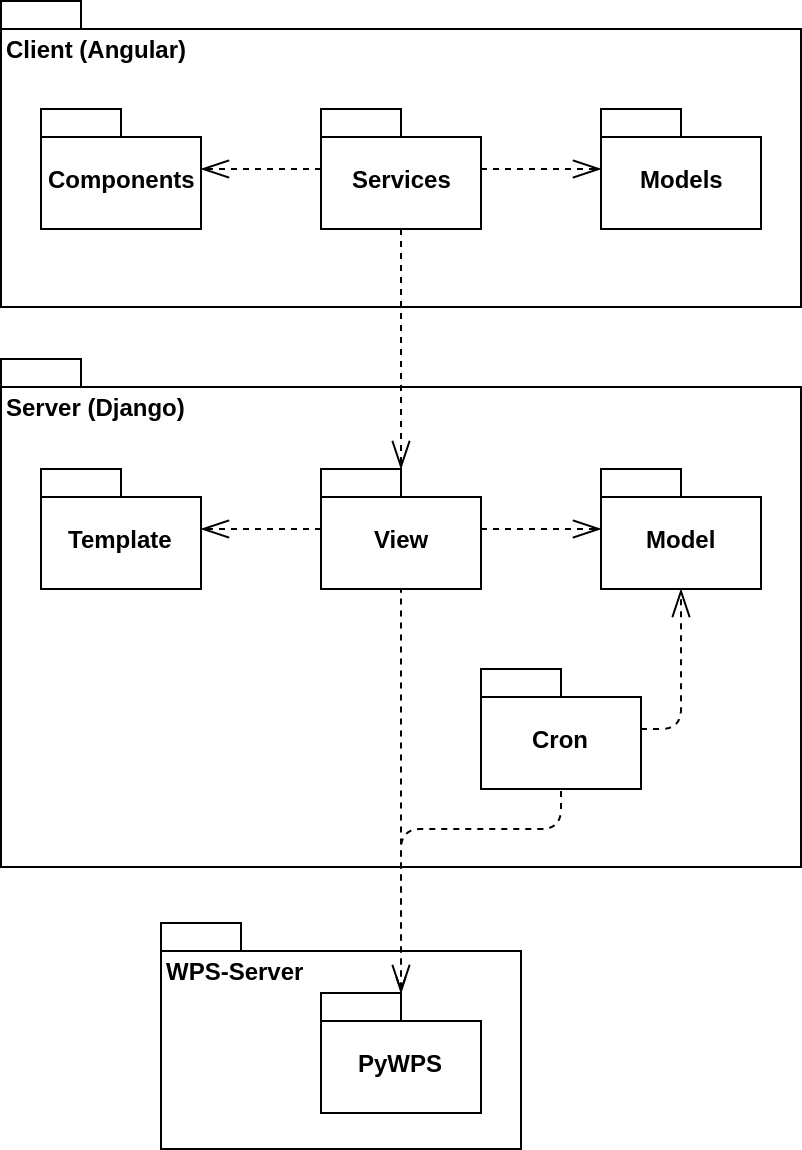
\includegraphics[width=8cm]{images/package_diagram.png}
        \caption{Paketdiagramm}
        \label{fig:arch_package_division}
    \end{figure}
    
        \subsection{Client}
        
        Der Client, der im Browser des Nutzers läuft, ist auf dem JavaScript-Framework Angular aufgebaut. Es wurde aus folgenden Gründen ausgewählt:
        
        \begin{itemize}
            \item Idee: Angular ist ein Framework das für Anwendungen verwendet wird die meist direkt im Browser laufen, was bei WPSflow genau der Fall ist
            \item Angular bietet für WPSflow wichtige Funktionalitäten an. Beispielsweise einen HTTPClient
            \item Eine hohe Qualität die durch eine große Community gewährleistet wird
            \item Es gibt eine Vielzahl von Erweiterungen
            \item Die interne Benutzung von TypeScript, welche es ermöglicht typisierten Code zu schreiben und dadurch einige Fehler zu vermeiden und die Produktivität der Implementierung zu steigern
        \end{itemize}

        \noindent Angular-Apps sind nach dem \gls{Model View Controller}-Prinzip (MVC) aufgebaut, wobei man für Views den Begriff Components verwendet und für Controller den Begriff Services. Models repräsentieren die Datenstrukturen. Components sind für das Anzeigen (auch Rendering genannt) zuständig und Services schicken Anfragen an den Server und empfangen die Antworten.
        
        \subsection{Server}
        
        Im dem Backend wird das Python-Framework \gls{Django} verwendet. Es benutzt einen modifizierten MVC-Ansatz, der deshalb andere Bezeichnungen verwendet Model - Template - View, kurz MTV.
        
        \begin{itemize}
            \item Model - Definiert Datenstrukturen und dient dem Zugriff auf die Datenbank
            \item View - Analog zum Controller im MVC
            
            \begin{itemize}
                \item Stellt REST-Schnittstelle zur Verfügung, die vom Client benutzt wird. Dieser Ansatz ermöglicht eine Wiederverwendbarkeit der API für zukünftige Apps - zum Beispiel Smartphone Apps
                \item Bearbeitet Abfragen vom Client und ruft Klassen aus dem Model-Paket auf um Daten zu holen oder zu schreiben
            \end{itemize}
            \item Template - Analog zu Views im MVC, enthält die HTML-Datei der Seiten 
            \item \gls{Cron} - wird in regelmäßigen Zeitabständen aufgerufen und fragt den Status des momentan ausgeführten Tasks beim WPS-Servern an. Falls ein Task erfolgreich beendet wurde, schickt der Cron ggf. den nächsten Task an den WPS-Server
        \end{itemize}
        
        \subsection{WPS-Server}
        
        Ein oder mehrere Server, die für die eigentlichen Berechnungen zuständig sind, werden extern zur Verfügung gestellt und in das System eingetragen. Der Server kommuniziert mit den externen Servern über das WPS Protokoll.
    